\begin{figure}[h]
    \centering
    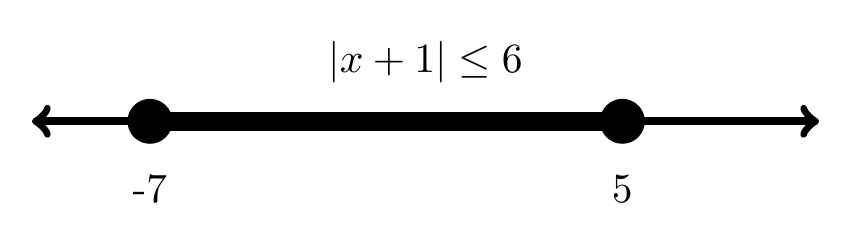
\begin{tikzpicture}[scale=0.5]
        %\draw [help lines] (-10,-10) grid (10,10);
        \draw [line width=3pt, <-] (-10,0) -- (-7.5,0);
        \draw [line width=7pt] (-7.5,0) -- (5.5,0);
        \draw [line width=3pt, ->] (5.5,0) -- (10,0);
        %\draw [line width=3pt, <->] (0,-10) -- (0,10);
        \draw [fill=black,line width=2pt] (5,0) circle [radius=0.5];
        \draw [fill=black,line width=2pt] (-7,0) circle [radius=0.5];
        \draw [fill=black,line width=3pt] (5, 0.5) -- (5,-0.5);
        \draw [fill=black,line width=3pt] (-7, 0.5) -- (-7,-0.5);
        
        %\draw [line width=2pt, fill=black] (4,4) circle [radius=0.1];
        \node [scale=1.5] at (0,1.5) {$|x+1| \leq 6$} ;
        \node [scale=1.5, below] at (5,-1) {5} ;
        \node [scale=1.5, below] at (-7,-1) {-7} ;
        
        %\draw [fill=black, line width=4pt] (5,7) circle [radius=.1];
        %\path [red, fill=blue, line width=5pt, |->] (-10,0) to [out=135,in=180] (0,7) to [out=0,in=45] (10,0);
    \end{tikzpicture}
    \caption{Vector image}
    \label{fig:my_label}
\end{figure}